% !TeX root = ../main.tex
% Background paradigm, not a method architecture or a four-task roadmap.
% Matrix: rows are representation levels (observation / 3D state),
% columns are time (t1 / t2=t / t+dt). Time runs left to right only.
% All photographs and model renders show the SAME PhysTwin cloth episode.
% State cutouts are pasted at one common cm/px scale, preserving the
% relative position of the two view-2 renders inside the 477x320 frame.
% Original JPEG panels, extraction map and SHA-256: materials/phystwin_cloth/.
% Axis, tau marker, arrows and labels are explanatory, not measured.
\begin{figure}[H]
  \centering
  \begingroup
  \definecolor{motInk}{HTML}{26343E}
  \definecolor{motMuted}{HTML}{6C7780}
  \definecolor{motLine}{HTML}{D8DDE1}
  \definecolor{motBlue}{HTML}{426A85}
  \definecolor{motAction}{HTML}{A66E38}
  \resizebox{\linewidth}{!}{%
  \begin{tikzpicture}[
    x=1cm,y=1cm,line cap=round,line join=round,text=motInk,
    font=\fontsize{9.5pt}{12pt}\selectfont,
    mothead/.style={font=\heiti\fontsize{10pt}{12pt}\selectfont},
    motnote/.style={font=\fontsize{8.5pt}{10.5pt}\selectfont,text=motMuted},
    rownote/.style={font=\fontsize{8pt}{9.6pt}\selectfont,text=motMuted},
    motarrow/.style={-{Latex[length=1.6mm,width=1.1mm]},draw=motBlue,line width=0.85pt},
    actarrow/.style={-{Latex[length=1.6mm,width=1.1mm]},draw=motAction,line width=0.9pt}
  ]
    \path[use as bounding box] (0,0) rectangle (15.6,7.10);

    % ---- time axis: it also serves as the column header ----
    \draw[motMuted!55,line width=0.5pt,-{Latex[length=1.3mm]}]
      (1.9,6.53) -- (15.15,6.53);
    \foreach \xx in {3.75,8.05,13.3}{%
      \draw[motMuted!70,line width=0.5pt] (\xx,6.53) -- (\xx,6.63);
    }
    \draw[motMuted!70,line width=0.5pt] (5.9,6.53) -- (5.9,6.63);
    \node at (3.75,6.78) {$t_1$};
    \node at (8.05,6.78) {$t_2=t$};
    \node at (13.3,6.78) {$t+\Delta t$};
    \node[motnote] at (5.9,6.78) {$\tau$};

    % ---- row labels: observation vs state ----
    \node[mothead] at (0.95,5.35) {视觉观测};
    \node[rownote] at (0.95,5.00) {离散、局部};
    \node[mothead] at (0.95,1.76) {三维状态};
    \node[rownote] at (0.95,1.41) {连续、可更新};

    % ---- observation row ----
    \node[anchor=north west,inner sep=0pt] at (1.9,6.383)
      {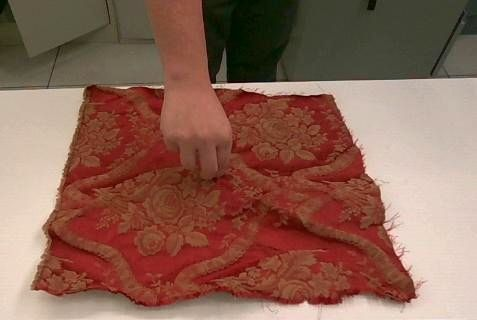
\includegraphics[width=3.7cm]{figures/materials/phystwin_cloth/observation_t1.jpg}};
    \draw[motLine,line width=0.35pt] (1.9,3.901) rectangle (5.6,6.383);
    \node[anchor=north west,inner sep=0pt] at (6.2,6.383)
      {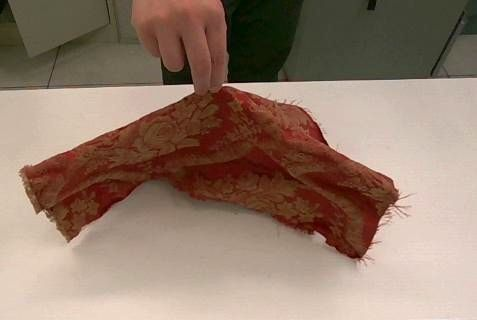
\includegraphics[width=3.7cm]{figures/materials/phystwin_cloth/observation_t2.jpg}};
    \draw[motLine,line width=0.35pt] (6.2,3.901) rectangle (9.9,6.383);
    \node[anchor=north west,inner sep=0pt] at (11.45,6.383)
      {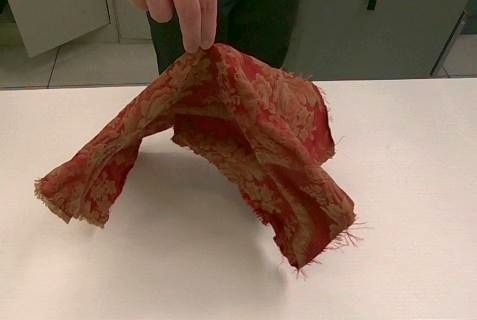
\includegraphics[width=3.7cm]{figures/materials/phystwin_cloth/execution_future.jpg}};
    \draw[dashed,motMuted!85,line width=0.55pt]
      (11.45,3.901) rectangle (15.15,6.383);

    % ---- state row: common scale k = 3.7cm / 280px ----
    % crop frame x=32..312, y=67..279 of the 477x320 renders
    \node[anchor=north west,inner sep=0pt] at (2.0057,2.5149)
      {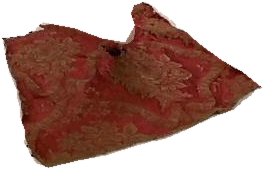
\includegraphics[width=3.4886cm]{figures/generated/world_model_paradigm/state_t1_view2_cutout.png}};
    \node[anchor=north west,inner sep=0pt] at (6.5832,2.8189)
      {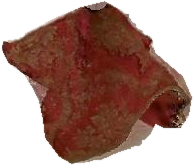
\includegraphics[width=2.5636cm]{figures/generated/world_model_paradigm/state_t2_view2_cutout.png}};
    \node[anchor=west,inner sep=0pt] at (11.45,1.5505)
      {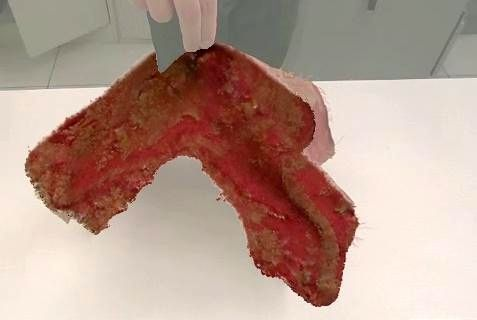
\includegraphics[width=3.7cm]{figures/materials/phystwin_cloth/prediction_future.jpg}};
    \draw[motLine,line width=0.35pt] (11.45,0.3095) rectangle (15.15,2.7915);
    % The prediction is a render of the same scene as the photographs; label it
    % explicitly so that it cannot be read as a captured frame.
    \node[anchor=south west,inner sep=2.2pt,fill=white,fill opacity=0.88,
      text opacity=1,font=\fontsize{8pt}{9.6pt}\selectfont]
      at (11.53,0.42) {模型预测};

    % ---- build / update the state from observations ----
    \draw[motarrow] (3.75,3.901) -- (3.75,2.951);
    \node[motnote,anchor=west] at (3.87,3.45) {构建};
    \draw[motarrow] (8.05,3.901) -- (8.05,2.951);
    \node[motnote,anchor=west] at (8.17,3.45) {更新};

    % ---- current state + given action -> forecast ----
    \draw[actarrow] (9.3,1.5505) -- (11.45,1.5505);
    \node[motnote,text=motAction] at (10.375,1.85) {给定动作 $\mathbf a$};

    % ---- the real future frame is a reference only, not an input ----
    \draw[dashed,motMuted,line width=0.6pt,
      {Latex[length=1.3mm]}-{Latex[length=1.3mm]}]
      (13.3,3.901) -- (13.3,2.7915);
    \node[motnote,anchor=west] at (13.42,3.45) {对照};

    % ---- tau: the state can be queried inside a sampling interval ----
    \draw[dashed,motMuted!55,line width=0.45pt] (5.9,6.53) -- (5.9,2.951);
    \fill[white] (5.9,2.951) circle (0.055);
    \draw[motMuted!55,line width=0.45pt] (5.9,2.951) circle (0.055);
    \node[motnote,anchor=west] at (6.02,3.19) {可查询};
  \end{tikzpicture}%
  }
  \endgroup
  \caption{连续动态世界模型的状态构建与演化预测概念示意（PhysTwin 案例素材）}
  \label{fig:dynamic-world-motivation}
\end{figure}
